% This work is licensed under the Creative Commons
% Attribution-NonCommercial-ShareAlike 4.0 International License. To view a copy
% of this license, visit http://creativecommons.org/licenses/by-nc-sa/4.0/ or
% send a letter to Creative Commons, PO Box 1866, Mountain View, CA 94042, USA.

% (c) Eric Kunze, 2019

%%%%%%%%%%%%%%%%%%%%%%%%%%%%%%%%%%%%%%%%%%%%%%%%%%%%%%%%%%%%%%%%%%%%%%%%%%%%%%%
% Template for lecture notes and exercises at TU Dresden.
%%%%%%%%%%%%%%%%%%%%%%%%%%%%%%%%%%%%%%%%%%%%%%%%%%%%%%%%%%%%%%%%%%%%%%%%%%%%%%%

\documentclass[ %
    ngerman, %
    a4paper, %
    sectionreset, %
    chapterstyle=framed, %
    sectionstyle=pure, %
    titlefont=osfamily %
]{../../texmf/tex/latex/mathscriptMathTUD/mathscriptMathTUD}

\usepackage[order=firstname, fractionappearence=lowerraise]{../../texmf/tex/latex/mathworkMathTUD/mathworkMathTUD}
%\usepackage[presentExercise]{../../texmf/tex/latex/exercisesMathTUD/exercisesMathTUD}

%%%%%%%%%%%%%%%%%%%%%%%%%%%%%%%%%%%%%%%%%%%%%%%%%%%%%%%%%%%%%%%%%%%%%%%%%%%%%%%

%---------------------------------------
% additional packages
%---------------------------------------

% none


%---------------------------------------
% general settings
%---------------------------------------

\name{Eric Kunze}
\matnr{Nummer}
\email{\href{mailto:eric.kunze@mailbox.tu-dresden.de}{\ttfamily eric.kunze@mailbox.tu-dresden.de}}

\modul{Stochastik}
\period{Sommersemester 2019}

%\renewcommand{\tutor}{Dr. Legrand}
%\renewcommand{\group}{Tag x. DS, (un)gerade Woche}

\lecturer{Prof. Dr. Anita Behme}
\faculty{Mathematik}
\institute{Stochastik}
\professorship{Angewandte Stochastik}

%%%%%%%%%%%%%%%%%%%%%%%%%%%%%%%%%%%%%%%%%%%%%%%%%%%%%%%%%%%%%%%%%%%%%%%%%%%%%%%

\counterwithin{themcount}{chapter}

\newcommand{\ereignisF}{\mathcal{F}}
\newcommand*{\WTheorie}{Wahrscheinlichkeitstheorie }
\newcommand*{\WMass}{Wahrscheinlichkeitsmaß }
\newcommand*{\WRaum}{Wahrscheinlichkeitsraum }
\newcommand*{\WRaeume}{Wahrscheinlichkeitsräume }
\newcommand*{\WVerteilung}{Wahrscheinlichkeitsverteilung }
\newcommand*{\Wkeit}{Wahrscheinlichkeit }
\newcommand*{\ZV}{Zufallsvariable}

%%%%%%%%%%%%%%%%%%%%%%%%%%%%%%%%%%%%%%%%%%%%%%%%%%%%%%%%%%%%%%%%%%%%%%%%%%%%%%%


\begin{document}

\MakeTitle[dark]
    
\tableofcontents

\setcounter{chapter}{-1}
\chapter{Einleitung}

\section*{Literatur}
\begin{itemize}[nolistsep]
    \item \textit{Georgii} : Stochastik (5. Auflage)
    \item \textit{Schilling} : Wahrscheinlichkeit
    \item \textit{Bauer} : Wahrscheinlichkeitstheorie (5. Auflage)
    \item \textit{Krengel} : Einführung in die W-Theorie und Statistik
    \item \textit{Dehling \& Haupt} : Einführung in die W-Theorie und Statistik
\end{itemize}

\section*{Was ist Stochastik ?}

Altgriechisch "Stochastikos" ($\sigma \tau  \chi \alpha \tau \iota \kappa  \zeta$) $\leadsto$ "scharfsinnig im Vermuten" % TODO

Fragestellungen stammen insbesondere aus dem Glücksspiel, heute vielmehr auch aus der Versicherungs- und Finanzmathematik - überall da, wo Zufall / Risiko / Chance auftaucht.

\subsection*{Was ist mathematische Stochastik ?}
\begin{itemize}[leftmargin=*]
    \item Beschreibt zufällige Phänomene in einer exakten Sprache. \\
    Bsp.: "Beim Würfeln erscheint jedes sechste Mal (im Schnitt) die Augenzahl 6" $\leadsto$ Gesetz der großen Zahlen
    \item lässt sich in zwei Teilgebiete unterteilen: Wahrscheinlichkeitstheorie \& Statistik \\
    Die W-Theorie beschreibt und untersucht konkret gegebene Zufallssituationen. Dagegen zieht die Statistik Schlussfolgerungen aus Beobachtungen. Dabei benötigt sie die Modelle der W-Theorie - umgekehrt benötigt auch die W-Theorie die Statistik zur Bestätigung der Modelle.
    \item In diesem Semester konzentrieren wir uns auf die Wahrscheinlichkeitstheorie.
\end{itemize}



\section{Wahrscheinlichkeitsräume}
\subsection*{Ergebnisraum}
Welche möglichen Ausgänge eines zufälligen Geschehens interessieren uns?
\begin{*beispiel}
    Würfeln: Augenzahl, aber nicht Lage, Fallhöhe, usw.
\end{*beispiel}

\begin{definition}[Ergebnisraum]
    Die Menge der relevanten Ergebnisse eines Zufallgeschehens nennen wir \begriff{Ergebnisraum} und bezeichnen diesen mit $\Omega$.
\end{definition}

\begin{*beispiel}
    \begin{itemize}
        \item Würfeln: $\Omega = \menge{1,2, \dots , 6}$
        \item Wartezeiten: $\Omega = \R_+ = [0,\infty)$ (also überabzählbar)
    \end{itemize}
\end{*beispiel}

\subsection*{Ereignisse}
Oft interessiert man sich gar nicht für das konkrete Ergebnis des Zufallsexperiments, sondern nur für das Eintreten gewisser Ereignisse.

\begin{*beispiel}
    Würfeln: Zahl ist $> 3$ \\
    Wartezeiten: Wartezeit ist $\leq 5$ Minuten
\end{*beispiel}

Wir wollen also Teilmengen des Ergebnisraums betrachten, d.h. Elemente von $\pows{\Omega}$ (Potenzmenge), denen eine Wahrscheinlichkeit zugeordnet werden kann d.h. welche \textit{messbar} sind.

\begin{definition}[Ereignisraum]
    Sei $\Omega \neq \emptyset$ ein Ergebnisraum und $\mathcal{F}$ eine $\sigma$-Algebra auf $\Omega$, d.h. eine Familie von Teilmengen von $\Omega$, sodass 
    \begin{enumerate}
        \item $\Omega \in \mathcal F$
        \item $A \in \mathcal{F} \follows A^\complement \in \mathcal{F}$
        \item $A_1, A_2, \dots \in \mathcal{F} \follows \bigcup_{i \geq 1} A_i \in \mathcal{F}$
    \end{enumerate}
    Dann heißt $(\Omega, \mathcal{F})$ \begriff{Ereignisraum} oder messbarer Raum.
\end{definition}

\subsection*{Wahrscheinlichkeit}
Wir ordnen nun den Ereignissen Wahrscheinlichkeiten mittels einer Abbildung $\abb{\mathbb{P}}{\mathcal{F}}{[0,1]}$
zu, sodass
\begin{enumerate}
    \item[(N)] Normierung: $\mathbb{P}(\Omega) = 1$
    \item[(A)] Additivität: Für paarweise disjunkte Ereignisse $A_1, A_2, \dots \in \mathcal{F}$ ist $\mathbb{P}\left(\bigcup_{i \geq 1} A_i\right) = \sum_{i \geq 0} \mathbb{P}(A_i)$.
\end{enumerate}

(N), (A) und die Nichtnegativität von $\mathbb{P}$ werden als Kolmogorov-Axiome bezeichnet (nach Kolmogorov: Grundbegriffe der Wahrscheinlichkeitstheorie, 1933).

\begin{definition}[Wahrscheinlichkeit]
    Sei $(\Omega, \mathcal{F})$ ein Ereignisraum und $\abb{\mathbb{P}}{\mathcal{F}}{[0,1]}$ eine Abbildung mit den Eigenschaften (N) und (A). Dann heißt $\mathbb{P}$ \begriff{Wahrscheinlichkeitsmaß} oder auch \begriff{Wahrscheinlichkeitsverteilung}.
\end{definition}

Aus der Definition folgen direkt die folgenden Eigenschaften:

\begin{satz}[Rechenregelen für Wahrscheinlichkeitsmaße] \label{satz: 1.4_rechenregeln}
    Sei $\mathbb{P}$ ein W-Maß auf einem Ereignisraum $(\Omega, \mathcal{F})$ und $A,B,A_1,A_2,\dots \in \mathcal{F}$. Dann gilt:
    \begin{enumerate}[leftmargin=*]
        \item $\mathbb{P}(\emptyset) = 0$
        \item Endliche Additivität: $\mathbb{P} (A \cup B) + \mathbb{P} (A \cap B) = \mathbb{P}(A) + \mathbb{P}(B)$ und $\mathbb{P}(A) + \mathbb{P}(A^\complement) = 1$
        \item Monotonie: $A \subseteq B \follows \mathbb{P}(A) \leq \mathbb{P}(B)$
        \item $\sigma$-Subadditivität: $\mathbb{P}\left(\bigcup_{i \geq 1} A_i \right)  \leq \sum_{i \geq 1} \mathbb{P}(A_i)$
        \item $\sigma$-Stetigkeit: Wenn $A_n \nearrow A$ (d.h. $A_1 \subseteq A_2 \subseteq \cdots$ und $A = \bigcup_{i=1}^{\infty}A_i$ ) oder $A_n \searrow A$, so gilt $\mathbb{P}(A_n) \to \mathbb{P}(A)$ für $n \to \infty$
    \end{enumerate}
\end{satz}
\begin{proof}
    siehe MINT oder Schillings Lehrbuch
\end{proof}

\begin{beispiel}
    Für einen beliebigen Ereignisraum $(\Omega, \mathcal{F})$ und ein beliebiges Element $\xi \in \Omega$ definiert
    \begin{align*}
        \delta_\xi(A) := \begin{cases} 1 & \xi \in A \\ 0 & \text{sonst} \end{cases}
    \end{align*}
    ein (degeneriertes) W-Maß auf $(\Omega, \mathcal{F})$, welches wir als \begriff{Dirac-Maß} oder Dirac-Verteilung bezeichnen.
\end{beispiel}

\begin{beispiel}
    Wir betrachten das Zufallsexperiment "Würfeln mit einem fairen, 6-seitigen Würfel" mit der Ergebnismenge $\Omega = \menge{1, \dots, 6}$ und Ereignisraum $\mathcal{F} = \pows{\Omega}$. Setzen wir aus Symmetriegründen
    \begin{align*}
        \mathbb{P}(A) = \frac{\# A}{6}
    \end{align*}
    mit $\# A = \card{A} = \text{Kardinalität}$. Dies definert ein W-Maß.
\end{beispiel}

\begin{beispiel}[Wartezeiten an der Bushaltestelle] \label{beispiel: 1_1.7_exponentialverteilung}
    Ergebnisraum $\Omega = \R_+$ und Ereignisraum Borel'sche $\sigma$-Algebra $\mathcal{F} = \mathcal{B}(\R_+)$. Ein mögliches W-Maß können wir durch
    \begin{align*}
        \mathbb{P}(A) \defeq \int_A \lambda e^{-\lambda x} \dx
    \end{align*}
    für einen Parameter $\lambda > 0$ festlegen. (offensichtlich gelten $\mathbb{P}(\Omega) = 1$ und die $\sigma$-Additivität aufgrund der $\sigma$-Additivität des Integrals). Wir bezeichnen dieses Maß als \begriff{Exponentialverteilung}. (Warum gerade dieses Maß für Wartezeiten gut geeigent ist, sehen wir später.)
\end{beispiel}

%%%%%%%%%%%%%%%%%%%%%%%%%%%%%%%%%%%%%%%%%%%%%%%%%%%%%%%%%%%%%%%%%%%%%%%%%%%%%%%%%%%%%
% TODO ÜBERARBEITEN

\begin{satz}[Konstruktion von WMaßen mit Dichten] \label{satz: 1.8_mass_mit_dichte}
    Sei $(\Omega, \ereignisF)$ ein Eriegnisraum.
    \begin{itemize}[leftmargin=*]
        \item $\Omega$ abzählbar, $\ereignisF = \pows{\Omega}$:  \\
        Sei $\rho = \left( \rho(\omega) \right)_{\omega \in \Omega}$ eine Folge in $[0,1]$ in $\sum_{\omega \in \Omega} \rho(\omega) = 1$, dann definiert
        \begin{equation*}
        \P(A) = \sum_{\omega \in A} \rho(\omega), \quad A \in \ereignisF
        \end{equation*}
        ein (diskretes) WMaß $\P$ auf $(\Omega, \ereignisF)$. $\rho$ wird als \begriff{Zähldichte} bezeichnet.
        Umgekehrt definiert jedes WMaß $\P$ auf $(\Omega, \ereignisF)$ mittels $\rho(\omega) = \P(\set{\omega}), \omega \in \Omega$ eine Folge $\rho$ mit den obigen Eigenschaften.
        \item $\Omega \subseteq \Rn, \ereignisF = \borel{\Omega}$: \\
        Sei $\abb{\rho}{\Omega}{[0, \infty)}$ eine Funktion, sodass
        \begin{enumerate}[nolistsep]
            \item $\int_{\Omega} \rho(x) \dx = 1$
            \item $\set{x \in \Omega \colon \rho(x) \leq c} \in \borel{\Omega}$ für alle $c > 0$ 
        \end{enumerate}
        dann definiert $\rho$ ein WMaß $\P$ auf $(\Omega, \ereignisF)$ durch 
        \begin{equation*}
            \P(A) = \int_{A} \rho(x) \dx = \int_{A} \rho \diff{\lambda}, \quad A \in \borel{\Omega}
        \end{equation*}
        Das Integral interpretieren wir stets als Lebesgue-Integral bzgl. Lebesgue-Maß $\lambda$.
        $\rho$ bezeichnet wir als \begriff{Dichte}, \begriff{Dichtefunktion} oder \begriff{Wahrscheinlichkeitsdichte} von $\P$ und nennen ein solches $\P$ (absolut) \begriff{stetig} (bzgl. dem Lebesgue-Maß).
    \end{itemize}
\end{satz}

\begin{proof}
    Der diskrete Fall ist klar.
    Im stetigen Fall folgt die Bahuptung aus den bekannten Eigenschaften des Lebesgue-Integrals ($\nearrow$ Schilling MINT, Lemma 8.9)
\end{proof}

\begin{*bemerkung}
    \begin{itemize}[leftmargin=*, nolistsep]
        \item Die eineindeutige Beziehung zwischen Dichte und Wahrscheinlichkeitsmaß überträgt sich nicht auf den stetigen Fall.
        \begin{itemize}[nolistsep]
            \item Nicht jedes Wahrscheinlichkeitsmaß auf $(\Omega, \borel{\Omega}), \Omega \subset \Rn$ besitzt eine Dichte.
            \item Zwei Dichtefunktionen definieren dasselbe Wahrscheinlichkeitsmaß, wenn sie sich nur auf einer Menge von Lebesgue-Maß $0$ unterscheiden.
        \end{itemize}
        \item Jede auf $\Omega \subset \Rn$ definierte Dichtefunktion $\rho$ lässt sich auf ganz $\Rn$ fortsetzen durch $\rho(x) = 0, x \notin \Omega$. Das erzeugte WMaß auf $(\Rn, \borel{\Rn})$ lässt mit den WMaß auf $(\Omega, \borel{\Omega})$ identifizieren.
        \item Mittels Dirac-Maß $\delta_{x}$ können auch jedes diskrete WMaß auf $\Omega \subset \Rn$ als WMaß auf $\Rn, \borel{\Rn}$ interpretieren:
        \begin{equation*}
            \P(A) = \sum_{\omega \in A} \rho(\omega) = \int_{A} \mathrm{d} \left( \sum_{\omega \in \Omega} \rho(\omega)\delta_{\omega} \right) \quad A \in \borel{\Rn}
        \end{equation*}
        \item stetige und diskrete WMaße lassen sich kombinieren z.B. definiert
        \begin{equation*}
            \P(A) = \frac{1}{2} \delta_{0} + \frac{1}{2} \int_{A} \one_{[0,1]}(x) \dx, A \in \borel{\R}
        \end{equation*}
        ein WMaß auf $(\R, \borel{\R})$.
    \end{itemize}
\end{*bemerkung}

Abschließend erinnern wir uns an:

\begin{satz}[Eindeutigkeitssatz für Wahrscheinlichkeitsmaße] \label{satz: 1.9_eindeutigkeitssatz}
    Sei $(\Omega, \ereignisF)$ Ereignisraum und $\P$ ein WMaß auf $(\Omega, \ereignisF)$. 
    Sei $\ereignisF = \omega(\mathcal{G})$ für ein $\cap$-stabiles Erzeugendensystem $\mathcal{G} \subset \pows{\Omega}$. 
    Dann ist $\P$ bereits durch seine Einschränkung $\P |_{\mathcal{G}}$ eindeutig bestimmt.
\end{satz}
\begin{proof}
    $\nearrow$ Schilling MINT, Satz 4.5.
\end{proof}

Insbesondere definiert z.B.
\begin{equation*}
    \P([0,a)) = \int_{0}^{a} \lambda e^{-\lambda x} \dx = 1 - e^{-\lambda a}, a > 0
\end{equation*}
bereits die Exponentialverteilung aus \cref{beispiel: 1_1.7_exponentialverteilung}.


\begin{definition}[Gleichverteilung] \label{def: 1.10_gleichverteilung}
    Ist $\Omega$ endlich, so heißt das WMaß mit konstanter Zähldichte 
    \begin{equation*}
        \rho(\omega) = \frac{1}{\abs{\Omega}}
    \end{equation*} 
    die \begriff{(diskrete) Gleichverteilung} auf $\Omega$ und wird mit $\Uni(\Omega)$ notiert (\textit{U = uniform}).
    
    Ist $\Omega \subset \Rn$ eine Borelmenge mit Lebesgue-Maß $0 < \lambda^n(\Omega) < \infty$ so heißt das WMaß auf $(\Omega, \borel(\Omega))$ mit konstanter Dichtefunktion 
    \begin{equation*}
        \rho(x) = \frac{1}{\lambda^n(\Omega)}
    \end{equation*} 
    die \begriff{(stetige)  Gleichverteilung} auf $\Omega$. 
    Sie wird ebenso mit $\Uni(\Omega)$ notiert.
\end{definition}

\subsection*{Wahrscheinlichkeitsräume}

\begin{definition}[Wahrscheinlichkeitsraum]
    Ein Tripel $(\Omega, \ereignisF, \P)$ mit $\Omega, \ereignisF$ Ereignisraum und $\P$ WMaß auf $(\Omega, \ereignisF)$, nennen wir \begriff{Wahrscheinlichkeitsraum}.
\end{definition}
\section{Zufallsvariablen}

Zufallsvariablen dienen dazu von einen gegebenen Ereignisraum $(\Omega, \ereignisF)$ zu einem Modellausschnitt $\Omega', \ereignisF'$ überzugehen. 
Es handelt sich also um Abbildungen $\abb{X}{\Omega}{\Omega'}$.
Damit wir auch jedem Ereignis in $\ereignisF'$ eine Wahrscheinlichkeit zuordnen können, benötigen wir	
\begin{equation*}
    A' \in \ereignisF' \follows X^{-1} A' \in \ereignisF		
\end{equation*}
d.h. $X$ sollte \begriff{messbar} sein.

\begin{definition}[Zufallsvariable]
    Seien $(\Omega, \ereignisF)$ und $(\Omega', \ereignisF')$ Ereignisräume. Dann heißt jede messbare Abbildung
    \begin{equation*}
        \abb{X}{\Omega}{\Omega'}
    \end{equation*}
    \begriff{Zufallsvariable} (von $(\Omega, \ereignisF)$) nach $(\Omega', \ereignisF')$/ auf $(\Omega', \ereignisF')$ oder \begriff{Zufallselement}.
\end{definition}

\begin{beispiel}
    \begin{enumerate}[leftmargin=*]
        \item Ist $\Omega$ abzählbar und $\ereignisF = \pows\Omega$, so ist jede Abbildung $\abb{X}{\Omega}{\Omega'}$ messbar und damit eine Zufallsvariable.
        \item Ist $\Omega \subset \Rn$ und $\ereignisF = \borel\Omega$, so ist jede stetige Funktion $\abb{X}{\Omega}{\R}$ messbar und damit eine Zufallsvariable.
    \end{enumerate}
\end{beispiel}

\begin{satz}
    Sei $(\Omega, \ereignisF, \P)$ ein \WRaum und $X$ eine Zufallsvariable von $(\Omega, \ereignisF)$ nach $(\Omega', \ereignisF')$. Dann definiert
    \begin{equation*}
    \P'(A') \defeq \P\left(X^{-1}(A')\right) = \P\left(\set{X \in A'}\right), \quad A' \in \ereignisF'
    \end{equation*}
    ein WMaß auf $(\Omega', \ereignisF')$, welches wir als \begriff{Wahrscheinlichkeitsverteilung von $X$ unter $\P$} bezeichnen.
\end{satz}

\begin{proof}
    Aufgrund der Messbarkeit von $X$ ist die Definition sinnvoll. Zudem gelten
    \begin{equation*}
        \P'(\Omega') = \P(X^{-1}(\Omega')) = \P(\Omega) = 1
    \end{equation*}
    und für $A_1', A_2', \dots \in \ereignisF'$ paarweise disjunkt.
    \begin{equation*}
    \begin{aligned}
        \P' \left( \bigcup_{i \geq 1} A_i' \right) 
        = \P \left(X^{-1}\left( \bigcup_{i \geq 1} A_i' \right) \right) 
        &= \P \left( \bigcup_{i \geq 1} X^{-1}(A_i') \right) \\
        &= \sum_{1 \geq 1} \P(X^{-1} A_i') \quad \text{ da auch } X^{-1}A_1', X^{-1}A_2', \dots \text{ paarweise disjunkt sind} \\
        &= \sum_{1 \geq 1} \P'(A_i)
    \end{aligned}
    \end{equation*}
    Also ist $\P'$ ein WMaß.
\end{proof}

\begin{*bemerkung}
    \begin{itemize}[leftmargin=*, nolistsep]
        \item Aus Gründen der Lesbarkeit schreiben wir in der Folge $\P (X \in A) = \P ( \menge{\omega \colon X(\omega) \in A} )$
        \item Ist $X$ die Identität, so fallen die Begriffe \WMass und \WVerteilung zusammen.
        \item In der (weiterführenden) Literatur zur \WTheorie wird oft auf die Angabe eines zugrundeliegenden WRaumes verzichtet und stattdessen eine ``Zufalsvariable mit Verteilung $\P$ auf $\Omega$'' eingeführt.
        Gemeint ist (fast) immer $X$ als Identität auf $(\Omega, \ereignisF, \P)$ mit $\ereignisF = \pows\Omega$ oder $\ereignisF = \borel\Omega$.
        \item Für die Verteilung von $X$ unter $\P$ schreibe $\P_X$ und $X \sim \P_{X}$ für die Tatsache, dass $X$ gemäß $\P_X$ verteilt ist.
    \end{itemize}
\end{*bemerkung}

\begin{definition}
    Zwei Zufallsvariablen sind \begriff{identisch verteilt}, wenn sie dieselbe Verteilung haben.
\end{definition}

Von besonderen Interesse sind für uns die Zufallsvariablen, die nach $(\R, \borel\R)$ abbilden, sogenannte \begriff{reelle Zufallsvariablen}.

Da die halboffenen Intervalle $\borel\R$ erzeugen, ist die Verteilung einer reellen Zufallsvariable durch die Werte $(-\infty, c]$, $c \in \R$ eindeutig festgelegt.

\begin{definition}[Verteilungsfunktion] \label{def: 1.16_verteilungsfunktion}
    Sei $(\R, \borel\R, \P)$ ein \WRaum, so heißt
    \begin{equation*}
        \abb{F}{\R}{[0,1]} \text{ mit } x \mapsto \P((-\infty, x))
    \end{equation*}
    \begriff{(kumulative) Verteilungsfunktion von $\P$}.    
    Ist $X$ eine reelle Zufallsvariable auf beliebigen WRaum $(\Omega, \ereignisF, \P)$, so heißt
    \begin{equation*}
        \abb{F}{\R}{[0,1]} \text{ mit } x \mapsto \P(X \leq x) = \P(X \in (-\infty, x])
    \end{equation*} % TODO everything good with the X's here?
    die (kumulative) Verteilungsfunktion von $X$.
\end{definition}

\begin{beispiel}
    $(\R, \borel\R,\P)$ mit $\P$ Exponentialverteilung mit Parameter $\lambda > 0$
    \begin{equation*}
    \P(A) = \int_{A \cap [0,\infty)}\lambda e^{-\lambda x} \dx \quad A \in \borel\R
    \end{equation*}
    Dann ist
    \begin{equation*}
    F(x) = \P((-\infty, x)) = 
    \begin{cases}
        0 &x \le 0\\
        \int_{0}^{x} \lambda e^{-\lambda y} \dy = 1 - e^{-\lambda x} &x > 0
    \end{cases}\notag
    \end{equation*}
\end{beispiel}

\begin{center}
    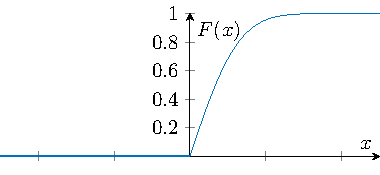
\includegraphics{./stoch_abbildungen/exponentialverteilung_verteilungsfunktion.pdf}
    \captionof{figure}{Verteilungsfunktion der Exponentialverteilung}
\end{center}

\begin{beispiel}
    Das Würfeln mit einem fairen, sechseitigen Würfel kann mittels einer reellen Zufallsvariablen
    \begin{equation*}
        \abb{X}{\menge{1,2,\dots, 6}}{\R} \mit x \mapsto x
    \end{equation*}
    modelliert werden. Es folgt als Verteilungsfunktion
    \begin{equation*}
    \begin{aligned}
    F(x) &= \P'(X \leq x) = \P(X^{-1}(-\infty,x]) = \P((-\infty,x]) \\
         &= \frac{1}{6}\sum_{i=1}^{6} \one_{\menge{i \leq x}}
    \end{aligned}
    \end{equation*}
\end{beispiel}

\begin{center}
    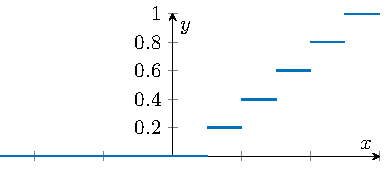
\includegraphics{./stoch_abbildungen/wuerfel_verteilungsfunktion.pdf}
    \captionof{figure}{Verteilungsfunktion des Würfelexperiments}
\end{center}

Diese Erkenntnisse lassen sich auch verallgemeinern:

\begin{satz}
    Ist $\P$ ein \WMass auf $(\R, \borel\R)$ und $F$ die zugehörige Verteilungsfunktion, so gelten
    \begin{enumerate}[nolistsep, topsep=-\parskip]
        \item $F$ ist monoton wachsend
        \item $F$ ist rechtsseitig stetig
        \item $\lim_{x\to -\infty} F(x) = 0$ und $\lim_{x\to \infty} F(x) = 1$
    \end{enumerate}
    Umgekehrt existiert zu jeder Funktion $\abb{F}{\R}{[0,1]}$ mit Eigenschaften (1) bis (3) eine reelle Zufallsvariable auf $((0,1), \borel((0,1)), \Uni((0,1))$ mit Verteilungsfunktion $F$.
\end{satz}

\begin{proof}
    Ist $F$ Verteilungsfunktion, so folgt mit \ref{satz: 1.4_rechenregeln}
    \begin{equation*}
        x \leq y \follows F(x) = \P((-\infty,x]) \overset{\ref{satz: 1.4_rechenregeln}.3}{\leq} \P((-\infty,y]) = F(y)
    \end{equation*}
    und
    \begin{equation*}
        \lim_{m \searrow c} F(x) = \lim_{m \searrow c} \P((-\infty, x]) \overset{\sigma\text{-Stetigkeit}}{=} \P((-\infty, c]) = F(c)
    \end{equation*}
    sowie
    \begin{equation*}
    \begin{aligned}
        \lim_{x\to -\infty} F(x) \overset{\ref{satz: 1.4_rechenregeln}.5}&{=} \P(\emptyset) \overset{\ref{satz: 1.4_rechenregeln}.1}{=} 0 \\
        \lim_{x\to \infty} F(x) \overset{\ref{satz: 1.4_rechenregeln}.5}&{=} \P(\R) = 1
    \end{aligned}
    \end{equation*}
    Umgekehrt wähle
    \begin{equation*}
        X(u) \defeq \inf \menge{x \in \R \colon F(x) \geq u}, \quad u \in (0,1)\\
    \end{equation*}
    Dann ist $X$ eine ``linkseitige Inverse'' von $F$ (auch \begriff{Quantilfunktion} oder \begriff{verallgemeinerte Inverse}).
    Wegen (3) gilt $-\infty < X(u) < \infty$ und zudem
    \begin{equation*}
        \menge{X \leq x} = (0, F(x)) \cap (0,1) \in \borel((0,1))
    \end{equation*}
    Da diese halboffene Mengen ein Erzeugendensystem von $\borel\R$ bilden, folgt bereits die Messbarkeit von $X$, also ist $X$ eine \ZV. Insbesondere hat die Menge $\menge{X \le x}$ gerade \person{Lebesgue}-Maß $F(x)$ und damit hat $X$ die Verteilungsfunktion $F$.
\end{proof}

\begin{korollar}
    Ist $\P$ \WMass auf $(\R, \borel\R)$ und $F$ die zugehörige Verteilungsfunktion. Dann besitzt $\P$ genau eine Dichtefunktion $\rho$, wenn $F$ stetig differenzierbar ist, denn dann gilt
    \begin{equation*}
        F(x) = \int_{0}^{x} \rho(x) \dx \quad \text{ bzw } \quad \rho(x) = F'(x)
    \end{equation*}
\end{korollar}

\begin{proof}
    Folgt aus \cref{satz: 1.8_mass_mit_dichte}, der \cref{def: 1.16_verteilungsfunktion} der Verteilungsfunktion und dem Eindeutigkeitssatz \labelcref{satz: 1.9_eindeutigkeitssatz}.
\end{proof}



\end{document}